% TorchWM — Technical Design & Progress Report
% Compile with: xelatex -interaction=nonstopmode torchwm_report.tex  (run twice)
\documentclass[10pt,a4paper]{article}

% ---------------------------------------------------------------- fonts ----
\usepackage{fontspec}
\setmainfont{Segoe UI}[
  BoldFont       = Segoe UI Bold,
  ItalicFont     = Segoe UI Italic,
  BoldItalicFont = Segoe UI Bold Italic,
  Ligatures      = TeX ]
\newfontfamily\displayfont{Segoe UI Semibold}[Ligatures=TeX]
\newfontfamily\lightfont{Segoe UI Light}[Ligatures=TeX]
\setmonofont{Consolas}[Scale=0.86]

% ------------------------------------------------------------- packages ----
\usepackage[a4paper,top=15mm,bottom=15mm,left=16mm,right=16mm,footskip=8mm]{geometry}
\usepackage{xcolor}
\usepackage{tikz}
\usetikzlibrary{positioning,arrows.meta,calc,fit,backgrounds,shapes.geometric,shadows.blur}
\usepackage[most]{tcolorbox}
\usepackage{listings}
\usepackage{booktabs}
\usepackage{array}
\usepackage{enumitem}
\usepackage{fancyhdr}
\usepackage{microtype}
\usepackage{multicol}
\usepackage[hidelinks]{hyperref}

\hypersetup{pdftitle={TorchWM: A Modular, Unified Framework for World Models and Embodied AI},
            pdfauthor={Param Thakkar}}

% --------------------------------------------------------------- colors ----
\definecolor{ink}{HTML}{101623}
\definecolor{body}{HTML}{2C3646}
\definecolor{muted}{HTML}{6E7A8C}
\definecolor{rule}{HTML}{DFE4EC}
\definecolor{panel}{HTML}{F5F7FB}
\definecolor{accent}{HTML}{2F5FE0}
\definecolor{accentsoft}{HTML}{E5ECFC}
\definecolor{amber}{HTML}{B26A00}
\definecolor{ambersoft}{HTML}{FBF0DC}
\definecolor{green}{HTML}{12734F}
\definecolor{greensoft}{HTML}{E1F1EA}
\definecolor{slate}{HTML}{55617A}
\definecolor{slatesoft}{HTML}{ECEFF5}
\definecolor{codebg}{HTML}{F7F8FA}

\color{body}

% --------------------------------------------------------- headers/foot ----
\pagestyle{fancy}
\fancyhf{}
\renewcommand{\headrulewidth}{0pt}
\renewcommand{\footrulewidth}{0pt}
\fancyfoot[L]{\footnotesize\color{muted}TorchWM \ \textbullet\ \ Technical Design \& Progress Report}
\fancyfoot[R]{\footnotesize\color{muted}\thepage\,/\,7}

% ------------------------------------------------------------- helpers -----
\setlength{\parindent}{0pt}
\setlength{\parskip}{0pt}

\newcommand{\kicker}[1]{{\footnotesize\displayfont\color{accent}\MakeUppercase{#1}}}

\newcommand{\pagetitle}[2]{%
  \kicker{#1}\par\vspace{1.5mm}
  {\Huge\displayfont\color{ink} #2}\par\vspace{2.5mm}
  {\color{rule}\hrule height 1pt}\par\vspace{4mm}}

\newcommand{\sectionhead}[1]{\vspace{1mm}{\large\displayfont\color{ink} #1}\par\vspace{2mm}}
\newcommand{\subhead}[1]{{\displayfont\color{ink} #1}\par\vspace{1mm}}

% status badges — used consistently throughout the document
\newcommand{\badge}[3]{\tcbox[on line,boxsep=0pt,left=3pt,right=3pt,top=1.4pt,bottom=1.4pt,
  boxrule=0pt,arc=2pt,colback=#1,coltext=#2]{\scriptsize\displayfont\MakeUppercase{#3}}}
\newcommand{\bimpl}{\badge{greensoft}{green}{implemented}}
\newcommand{\bprog}{\badge{ambersoft}{amber}{in progress}}
\newcommand{\bprop}{\badge{accentsoft}{accent}{proposed}}
\newcommand{\bvis}{\badge{slatesoft}{slate}{vision}}

\newtcolorbox{callout}[1][]{enhanced,breakable,colback=panel,colframe=rule,boxrule=0.6pt,
  arc=2pt,left=4mm,right=4mm,top=2.6mm,bottom=2.6mm,#1}
\newtcolorbox{accentcallout}[1][]{enhanced,colback=accentsoft,colframe=accentsoft,boxrule=0pt,
  arc=2pt,left=4mm,right=4mm,top=2.8mm,bottom=2.8mm,
  borderline west={1.4pt}{0pt}{accent},#1}
\newtcolorbox{warncallout}[1][]{enhanced,colback=ambersoft,colframe=ambersoft,boxrule=0pt,
  arc=2pt,left=4mm,right=4mm,top=2.8mm,bottom=2.8mm,
  borderline west={1.4pt}{0pt}{amber},#1}

\setlist[itemize]{leftmargin=3.6mm,itemsep=1.0mm,topsep=1.0mm,parsep=0pt,label=\textcolor{accent}{\scriptsize$\bullet$}}

% ------------------------------------------------------------- listings ----
\lstdefinestyle{py}{
  language=Python,
  basicstyle=\ttfamily\scriptsize\color{body},
  keywordstyle=\color{accent},
  commentstyle=\color{muted}\itshape,
  stringstyle=\color{green},
  showstringspaces=false,
  breaklines=true,
  frame=none,
  backgroundcolor=\color{codebg},
  xleftmargin=3mm, xrightmargin=1mm,
  framexleftmargin=3mm,
  aboveskip=1.5mm, belowskip=1.5mm,
  columns=fullflexible,
  keepspaces=true,
  morekeywords={as,with,import,from,for,in,def,class,return,None,True,False}
}
\lstset{style=py}

% tikz styles
\tikzset{
  lbox/.style={draw=rule,fill=white,rounded corners=1.6pt,line width=0.5pt,
               inner sep=1.6mm,align=center,font=\scriptsize},
  abox/.style={lbox,draw=accent!45,fill=accentsoft},
  gbox/.style={lbox,draw=green!45,fill=greensoft},
  mbox/.style={lbox,draw=amber!45,fill=ambersoft},
  sbox/.style={lbox,draw=slate!35,fill=slatesoft},
  band/.style={draw=rule,fill=panel,rounded corners=2.5pt,line width=0.5pt},
  arr/.style={-{Stealth[length=1.6mm,width=1.4mm]},draw=slate,line width=0.6pt},
  lbl/.style={font=\scriptsize\displayfont,color=ink,align=left},
  tiny/.style={font=\tiny,color=muted}
}

\begin{document}

% =========================================================== PAGE 1 =========
\thispagestyle{fancy}

\begin{tikzpicture}[remember picture,overlay]
  \fill[ink] ([xshift=0mm,yshift=0mm]current page.north west)
    rectangle ([xshift=0mm,yshift=-86mm]current page.north east);
  \fill[accent] ([xshift=0mm,yshift=-86mm]current page.north west)
    rectangle ([xshift=0mm,yshift=-87.2mm]current page.north east);
\end{tikzpicture}

\vspace*{5mm}
{\color{white}
  {\footnotesize\displayfont\color{accent!35!white}TECHNICAL DESIGN \& PROGRESS REPORT \quad\textbullet\quad AUGUST 2026}\par
  \vspace{6mm}
  {\fontsize{40}{44}\selectfont\displayfont TorchWM}\par
  \vspace{3mm}
  {\fontsize{14.5}{18}\selectfont\lightfont\color{white}A Modular, Unified Framework for\\World Models and Embodied AI}\par
  \vspace{7mm}
  {\large\displayfont\color{accent!35!white}“Build once. Experiment across world models.”}\par
  \vspace{6mm}
  {\footnotesize\color{white!62!ink}Param Thakkar \quad\textbullet\quad \texttt{github.com/ParamThakkar123/torchwm} \quad\textbullet\quad MIT licensed \quad\textbullet\quad Open source}
}
\vspace{12mm}

% ---- what it is
\sectionhead{What TorchWM is}
TorchWM is an open-source PyTorch library that brings the major world-model families (recurrent
state-space models, transformer/token-based models, diffusion models, and joint-embedding predictive
architectures) under one consistent API, together with the environments, datasets, training loops,
export paths, and evaluation harnesses they need. Its ambition is to be the layer beneath
world-model and embodied-AI research: the place where a \emph{dynamics model}, an \emph{encoder},
an \emph{environment}, and a \emph{policy} are independently replaceable parts rather than
assumptions baked into a single research repository.

\vspace{3mm}
{\color{rule}\hrule height 0.6pt}
\vspace{3.5mm}

% ---- three columns
\begin{minipage}[t]{0.315\textwidth}
  \kicker{The problem}\par\vspace{1.5mm}
  {\footnotesize
  World-model research is fragmented at the infrastructure layer. Each influential paper ships its
  own dataset format, environment wrapper, model definition, training loop, config system, and
  evaluation script. Reproducing a result, comparing two methods fairly, or combining an encoder
  from one paper with a dynamics model from another is an engineering project before it is a
  research question.}
\end{minipage}\hfill
\begin{minipage}[t]{0.315\textwidth}
  \kicker{Why it matters}\par\vspace{1.5mm}
  {\footnotesize
  A world model is a learned simulator: it predicts how an environment evolves in response to
  actions. That single capability underwrites sample-efficient model-based RL, planning in latent
  space, and embodied agents that can rehearse before acting in the physical world. It is one of
  the few places where perception, action, and prediction have to be solved jointly, and it is
  moving fast.}
\end{minipage}\hfill
\begin{minipage}[t]{0.315\textwidth}
  \kicker{The long-term vision}\par\vspace{1.5mm}
  {\footnotesize
  What PyTorch did for differentiable computation and Gymnasium did for environment interfaces,
  TorchWM aims to do for world models: a small set of durable abstractions that absorb the
  infrastructure work, stay out of the way of research, and let a new idea be tested against many
  models, datasets, and environments without rewriting the scaffolding around it.}
\end{minipage}

\vspace{5mm}

% ---- status strip
\begin{callout}
  \subhead{Where the project actually stands today}
  {\footnotesize
  TorchWM is early. It is a working library with a broad implemented surface and a single primary
  maintainer, not an established piece of ecosystem infrastructure. It has no published benchmark
  results, no measured adoption to report, and no external contributors beyond incidental patches.}
  \vspace{2.5mm}

  {\centering
  \begin{tabular}{@{}p{0.155\textwidth}p{0.155\textwidth}p{0.155\textwidth}p{0.155\textwidth}p{0.155\textwidth}p{0.145\textwidth}@{}}
  {\Large\displayfont\color{ink}0.4.2} & {\Large\displayfont\color{ink}13} & {\Large\displayfont\color{ink}11} & {\Large\displayfont\color{ink}819} & {\Large\displayfont\color{ink}593} & {\Large\displayfont\color{ink}52}\\[0.6mm]
  {\tiny\color{muted}latest PyPI release\newline (0.5.0 unreleased)} &
  {\tiny\color{muted}registered model\newline families} &
  {\tiny\color{muted}environment\newline backends} &
  {\tiny\color{muted}tests collected\newline in \texttt{tests/}} &
  {\tiny\color{muted}commits since\newline Nov 2025} &
  {\tiny\color{muted}documentation\newline pages}\\
  \end{tabular}\par}
\end{callout}

\vspace{3mm}

\begin{accentcallout}
  {\footnotesize\subhead{How to read this document}
  TorchWM is early-stage, and this report is explicit about the boundary between what exists and
  what is designed. Three markers are used consistently on every page that follows:\par\vspace{1.5mm}
  \bimpl\ working code in the repository today \quad
  \bprog\ partially built \quad
  \bprop\ designed, not yet built \quad
  \bvis\ long-term direction\par\vspace{1.5mm}
  Nothing marked \textsc{proposed} or \textsc{vision} should be read as shipped.}
\end{accentcallout}

\newpage
% =========================================================== PAGE 2 =========
\pagetitle{The problem}{Fragmented world-model research}

{\footnotesize
Every serious world-model result of the last few years arrived as a self-contained research
codebase. Each one is internally coherent and externally incompatible with the others. The
duplication is not in the ideas; it is in everything underneath them.}

\vspace{4mm}

% ---- silo diagram
\begin{center}
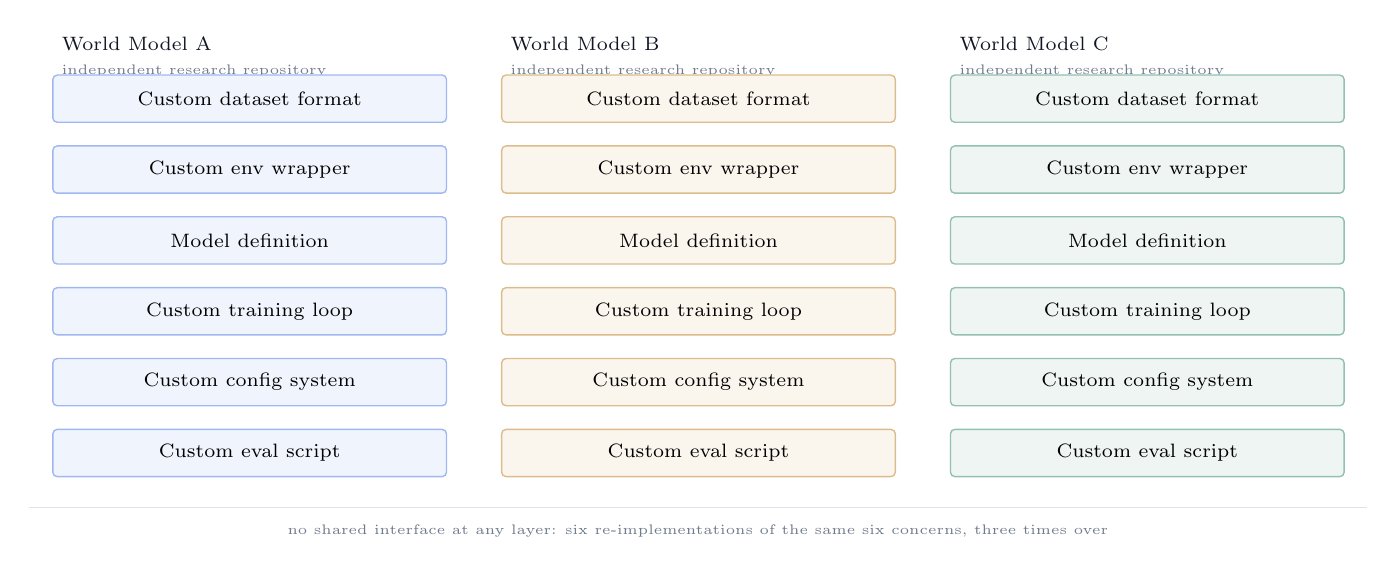
\begin{tikzpicture}[x=1mm,y=1mm]
  \def\cw{50}   % column width
  \def\rh{9}    % row height
  \foreach \i/\x/\name/\col in {0/0/{World Model A}/accent, 1/57/{World Model B}/amber, 2/114/{World Model C}/green}{
    \node[lbl,anchor=north west] at (\x,4) {\name};
    \node[tiny,anchor=north west] at (\x,0.5) {independent research repository};
    \foreach \j/\lay in {0/{Custom dataset format}, 1/{Custom env wrapper}, 2/{Model definition},
                         3/{Custom training loop}, 4/{Custom config system}, 5/{Custom eval script}}{
      \node[lbox,draw=\col!45,fill=\col!7,minimum width=\cw mm,minimum height=6mm,anchor=north west]
        at (\x, -2 - \j*\rh) {\lay};
    }
  }
  % duplication brackets
  \draw[rule,line width=0.6pt] (-3,-57) -- (167,-57);
  \node[tiny,anchor=north] at (82,-58) {no shared interface at any layer: six re-implementations of the same six concerns, three times over};
\end{tikzpicture}
\end{center}

\vspace{2mm}

% ---- consequences
\begin{center}
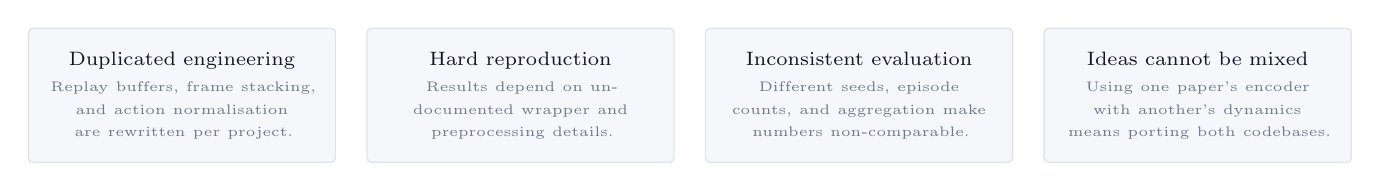
\begin{tikzpicture}[x=1mm,y=1mm]
  \foreach \i/\t/\d in {0/{Duplicated engineering}/{Replay buffers, frame stacking, and action normalisation are rewritten per project.},
                        1/{Hard reproduction}/{Results depend on undocumented wrapper and preprocessing details.},
                        2/{Inconsistent evaluation}/{Different seeds, episode counts, and aggregation make numbers non-comparable.},
                        3/{Ideas cannot be mixed}/{Using one paper's encoder with another's dynamics means porting both codebases.}}{
    \node[lbox,fill=panel,draw=rule,minimum width=39mm,minimum height=17mm,anchor=north west,text width=35mm]
      at (\i*43, 0) {{\displayfont\color{ink}\t}\\[0.6mm]{\tiny\color{muted}\d}};
  }
\end{tikzpicture}
\end{center}

\vspace{3mm}

\begin{callout}
  {\footnotesize
  \subhead{This is documented, not assumed}
  The fragmentation problem is recognised in the literature. \emph{stable-worldmodel} (Maes et al.)
  observes that world-model research ``remains fragmented and lacks shared benchmarks comparable to
  those in vision, reinforcement learning, or language modeling,'' and points to two contemporary
  works that independently re-implemented the same Two-Room environment with substantial divergence
  : a concrete case where the absence of shared infrastructure directly damaged comparability
  [4]. Recent surveys of world models for embodied AI reach the same conclusion about evaluation
  [6, 7].}
\end{callout}

\vspace{4mm}
\sectionhead{Before TorchWM \, vs. \, with TorchWM}

\begin{center}
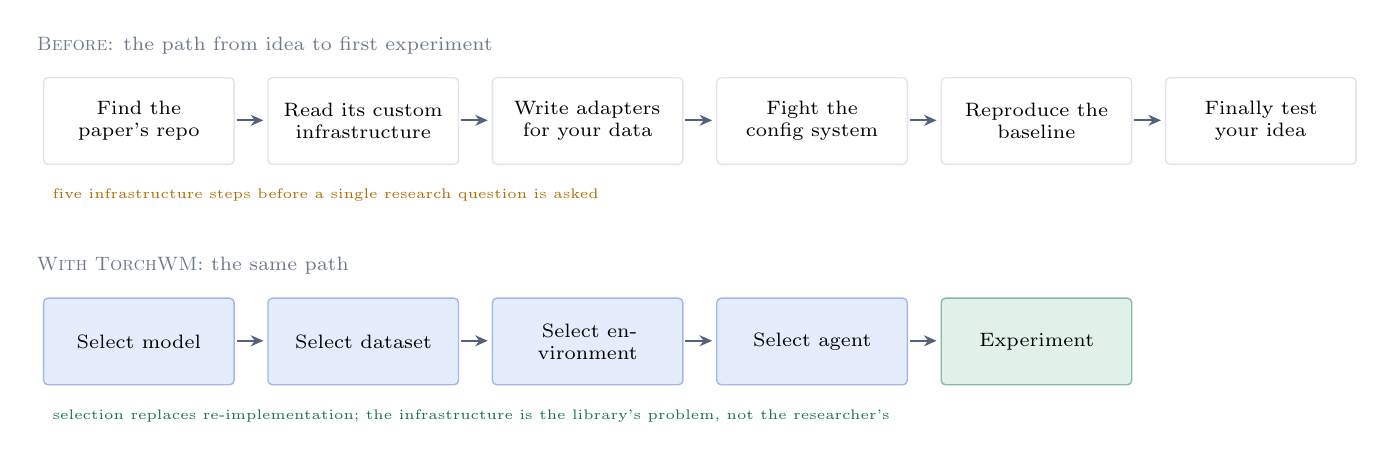
\begin{tikzpicture}[x=1mm,y=1mm]
  % --- BEFORE
  \node[lbl,anchor=west,color=muted] at (-2,4) {\textsc{Before}: the path from idea to first experiment};
  \foreach \i/\t in {0/{Find the\\ paper's repo}, 1/{Read its custom\\ infrastructure}, 2/{Write adapters\\ for your data},
                     3/{Fight the\\ config system}, 4/{Reproduce the\\ baseline}, 5/{Finally test\\ your idea}}{
    \node[lbox,fill=white,draw=rule,minimum width=24mm,minimum height=11mm,anchor=north west,text width=21mm]
      at (\i*28.5, 0) {\t};
    \ifnum\i<5 \draw[arr] (\i*28.5+24.6,-5.5) -- (\i*28.5+28,-5.5); \fi
  }
  \node[tiny,anchor=north west,color=amber] at (0,-13) {five infrastructure steps before a single research question is asked};

  % --- AFTER
  \node[lbl,anchor=west,color=muted] at (-2,-24) {\textsc{With TorchWM}: the same path};
  \foreach \i/\t/\c in {0/{Select model}/accent, 1/{Select dataset}/accent, 2/{Select environment}/accent, 3/{Select agent}/accent}{
    \node[lbox,draw=accent!45,fill=accentsoft,minimum width=24mm,minimum height=11mm,anchor=north west,text width=21mm]
      at (\i*28.5, -28) {\t};
    \draw[arr] (\i*28.5+24.6,-33.5) -- (\i*28.5+28,-33.5);
  }
  \node[lbox,draw=green!50,fill=greensoft,minimum width=24mm,minimum height=11mm,anchor=north west,text width=21mm]
    at (114, -28) {{\displayfont Experiment}};
  \node[tiny,anchor=north west,color=green] at (0,-41) {selection replaces re-implementation; the infrastructure is the library's problem, not the researcher's};
\end{tikzpicture}
\end{center}

\vspace{3mm}
{\footnotesize
The claim is specific. TorchWM removes the incidental difficulty (the adapters, wrappers, loops,
and config systems) so that the remaining difficulty is the research itself: representation,
dynamics, and control. That is the part worth a researcher's time.}

\newpage
% =========================================================== PAGE 3 =========
\pagetitle{Architecture}{Standard contracts, replaceable parts}

{\footnotesize
The architecture is a stack of layers, each defined by a contract rather than an implementation.
A layer's job is to specify what crosses its boundary (observations, latent states, actions,
predicted transitions, metrics) so that anything satisfying the contract can be substituted.
Boxes below reflect components that exist in the repository today unless marked otherwise.}

\vspace{3.5mm}

\begin{center}
\begin{tikzpicture}[x=1mm,y=1mm,font=\scriptsize]
  \def\bx{20}      % band x start
  \def\bw{116}     % band width
  \def\gap{15.4}   % row pitch

  % ---- cross-cutting spine (left): contracts
  \node[band,fill=accentsoft,draw=accent!35,minimum width=15mm,minimum height=104mm,anchor=north west] at (0,0) {};
  \node[rotate=90,anchor=center,font=\scriptsize\displayfont,color=accent] at (7.5,-52)
    {TorchWM contracts};
  \node[rotate=90,anchor=center,font=\tiny,color=accent!75!black,text width=95mm,align=center] at (12.2,-52)
    {ModelSpec \ \textbullet\ \ EnvBackendSpec \ \textbullet\ \ \texttt{info}-dict step contract \ \textbullet\ \ config dataclasses \ \textbullet\ \ plugin registry};

  % ---- cross-cutting spine (right): services
  \node[band,fill=slatesoft,draw=slate!30,minimum width=25mm,minimum height=104mm,anchor=north west] at (145,0) {};
  \node[anchor=north,font=\scriptsize\displayfont,color=slate,text width=23mm,align=center] at (157.5,-2)
    {Cross-cutting services};
  \foreach \j/\s in {0/{Configuration},1/{Training loops},2/{Checkpoints},3/{Logging (TB/W\&B)},
                     4/{Metrics \& reporting},5/{Model registry},6/{Env adapters},7/{Export: ONNX /\\TorchScript / TensorRT}}{
    \node[lbox,fill=white,draw=slate!25,minimum width=21mm,anchor=north,text width=18mm,font=\tiny]
      at (157.5,-9.5-\j*11.6) {\s};
  }

  % ---- layer bands
  \foreach \i/\name/\impls in {
    0/{Environment / Dataset}/{},
    1/{Observation \& action interfaces}/{},
    2/{Encoder / representation}/{},
    3/{World model / dynamics}/{},
    4/{Planner / policy}/{},
    5/{Embodied agent}/{},
    6/{Evaluation / benchmarks}/{}}{
    \node[band,minimum width=\bw mm,minimum height=12.4mm,anchor=north west] at (\bx,-\i*\gap-1) {};
    \node[anchor=north west,font=\tiny\displayfont,color=ink] at (\bx+2,-\i*\gap-1.6) {\name};
    \ifnum\i<6 \draw[arr] (\bx+\bw/2,-\i*\gap-13.6) -- (\bx+\bw/2,-\i*\gap-16.0); \fi
  }

  % row 0 — envs / datasets
  \foreach \k/\t in {0/{Gym / Gymnasium}, 1/{Atari (ALE)}, 2/{DM Control}, 3/{MuJoCo · Brax}, 4/{Rollout \&\\video datasets}}{
    \node[gbox,minimum width=20mm,minimum height=6mm,anchor=north west,text width=17mm,font=\tiny]
      at (\bx+2+\k*22.5,-6.2) {\t};
  }
  % row 1 — obs/action interfaces
  \foreach \k/\t in {0/{\texttt{terminated} /\\\texttt{truncated} / \texttt{discount}}, 1/{action\\normalisation}, 2/{pixel \& vector\\observations}, 3/{vectorised envs}}{
    \node[gbox,minimum width=20mm,minimum height=6mm,anchor=north west,text width=17mm,font=\tiny]
      at (\bx+2+\k*22.5,-6.2-\gap) {\t};
  }
  \node[mbox,minimum width=20mm,minimum height=6mm,anchor=north west,text width=17mm,font=\tiny]
      at (\bx+2+4*22.5,-6.2-\gap) {multimodal\\observations};
  % row 2 — encoders
  \foreach \k/\t in {0/{Conv encoder\\(Dreamer)}, 1/{PlaNet encoder}, 2/{ViT / JEPA}, 3/{VQ-VAE\\tokeniser}, 4/{Video\\tokeniser}}{
    \node[gbox,minimum width=20mm,minimum height=6mm,anchor=north west,text width=17mm,font=\tiny]
      at (\bx+2+\k*22.5,-6.2-2*\gap) {\t};
  }
  % row 3 — dynamics
  \foreach \k/\t in {0/{RSSM /\\ModularRSSM}, 1/{MDN-RNN}, 2/{Transformer\\(IRIS)}, 3/{Diffusion\\(DIAMOND · DiT)}, 4/{Spatiotemporal\\(Genie)}}{
    \node[gbox,minimum width=20mm,minimum height=6mm,anchor=north west,text width=17mm,font=\tiny]
      at (\bx+2+\k*22.5,-6.2-3*\gap) {\t};
  }
  % row 4 — planner/policy
  \foreach \k/\t in {0/{CEM planner\\(PlaNet)}, 1/{Latent-imagination\\actor–critic}, 2/{PPO harness}, 3/{IRIS policy}, 4/{Latent-action\\model (Genie)}}{
    \node[gbox,minimum width=20mm,minimum height=6mm,anchor=north west,text width=17mm,font=\tiny]
      at (\bx+2+\k*22.5,-6.2-4*\gap) {\t};
  }
  % row 5 — agents
  \foreach \k/\t in {0/{Dreamer v1/v2/v3}, 1/{PlaNet}, 2/{IRIS}, 3/{DIAMOND · DiT}, 4/{Genie · JEPA}}{
    \node[gbox,minimum width=20mm,minimum height=6mm,anchor=north west,text width=17mm,font=\tiny]
      at (\bx+2+\k*22.5,-6.2-5*\gap) {\t};
  }
  % row 6 — eval
  \foreach \k/\t in {0/{Atari-100k\\harness}, 1/{FID · FVD ·\\LPIPS · PSNR}, 2/{IQM +\\bootstrap CI}, 3/{JSON / CSV /\\Markdown reports}}{
    \node[gbox,minimum width=20mm,minimum height=6mm,anchor=north west,text width=17mm,font=\tiny]
      at (\bx+2+\k*22.5,-6.2-6*\gap) {\t};
  }
  \node[mbox,minimum width=20mm,minimum height=6mm,anchor=north west,text width=17mm,font=\tiny]
      at (\bx+2+4*22.5,-6.2-6*\gap) {cross-model\\leaderboard};

  % legend
  \node[gbox,minimum width=3mm,minimum height=2.6mm,anchor=west] at (20,-110) {};
  \node[anchor=west,font=\tiny,color=muted] at (25,-110) {implemented in the repository};
  \node[mbox,minimum width=3mm,minimum height=2.6mm,anchor=west] at (78,-110) {};
  \node[anchor=west,font=\tiny,color=muted] at (83,-110) {designed / partially built};
\end{tikzpicture}
\end{center}

\vspace{1mm}

\sectionhead{The contracts that make substitution work}
{\footnotesize
Modularity is only real if it is enforced somewhere. In TorchWM it is enforced by four concrete
mechanisms, all of which exist today:}

\vspace{2mm}
{\footnotesize
\begin{tabular}{@{}p{0.235\textwidth}p{0.50\textwidth}p{0.20\textwidth}@{}}
\toprule
\textbf{Contract} & \textbf{What it guarantees} & \textbf{Status}\\
\midrule
\texttt{ModelSpec} & Name, import path, config class, and aliases for every model family, so \texttt{create\_model("iris")} works identically to \texttt{create\_model("dreamer-v3")}. & \bimpl\\[1.2mm]
\texttt{EnvBackendSpec} & Name and factory path per backend, so \texttt{make\_env(id, backend=...)} is uniform across Gym, ALE, DMC, MuJoCo, Brax, Procgen, DMLab, bsuite, and Unity. & \bimpl\\[1.2mm]
\texttt{info}-dict step contract & Every adapter and wrapper normalises \texttt{step()} to always return \texttt{terminated}, \texttt{truncated}, and \texttt{discount}, verified by cross-backend contract tests. & \bimpl\\[1.2mm]
Plugin registry & \texttt{register\_world\_model} / \texttt{register\_env\_backend} let external packages appear in \texttt{list\_models()} and the factory API without patching TorchWM. & \bimpl\\
\bottomrule
\end{tabular}}

\vspace{2.5mm}
\begin{callout}
{\footnotesize
\subhead{One design decision worth calling out: the world model \emph{is} an environment}
\texttt{WorldModelEnv} wraps a trained dynamics model behind the standard \texttt{gym.Env}
interface. A latent rollout therefore looks exactly like environment interaction, which means any
policy-optimisation code (TorchWM's own actor–critic and PPO harness, or an external RL library)
can train inside an imagined world without knowing it is imagined. This is the single abstraction
that connects the model-learning half of the stack to the control half. \bimpl}
\end{callout}

\newpage
% =========================================================== PAGE 4 =========
\pagetitle{Researcher experience}{What using TorchWM looks like}

{\footnotesize
The API's design goal is that swapping a model family, an environment backend, or a component
inside a model should be an edit to a string or a constructor argument, not a fork.}

\vspace{3.5mm}

\begin{minipage}[t]{0.485\textwidth}
  \subhead{\bimpl\ \ Working today}
  {\footnotesize The following runs against the current package. Construction is unified across all
  13 registered model families; the shared step-budget \texttt{train()} currently covers the
  Dreamer family, which is discussed honestly on the next page.}
  \vspace{1.5mm}
\begin{lstlisting}
import torchwm

# Discover what the registry exposes.
torchwm.list_models()
# ['diamond', 'dit', 'dreamer', 'dreamer-v1',
#  'dreamer-v2', 'dreamer-v3', 'genie', ...]

# One factory, every model family.
agent = torchwm.create_model(
    "dreamer-v3",
    env="walker-walk",     # DeepMind Control
    env_backend="dmc",
    total_steps=1_000_000,
)
agent.train()

# Environments through one backend selector.
env = torchwm.make_env("ALE/Pong-v5",
                       backend="atari")

# Swap the algorithm, keep the code.
for algo in ["dreamer-v1", "dreamer-v2",
             "dreamer-v3"]:
    torchwm.create_model(
        algo, env="Pendulum-v1",
        env_backend="gym", total_steps=20_000
    ).train()
\end{lstlisting}
  \vspace{1mm}
  {\footnotesize\subhead{\bimpl\ \ Composing below the factory}}
\begin{lstlisting}
from torchwm import DreamerAgent, ConvEncoder
from torchwm.models import ModularRSSM
from torchwm.envs import WorldModelEnv

# A trained dynamics model, used as a gym.Env:
# latent rollouts drive ordinary RL code.
imagined = WorldModelEnv(model=world_model)
\end{lstlisting}
\end{minipage}\hfill
\begin{minipage}[t]{0.485\textwidth}
  \subhead{\bprop\ \ Proposed interface: not yet implemented}
  {\footnotesize The unified \texttt{Trainer} / \texttt{evaluate} surface below is a design target.
  The pieces it would sit on (registry, env adapters, benchmark runner, metrics) exist; the
  single entry point that composes them does not.}
  \vspace{1.5mm}
\begin{lstlisting}
# PROPOSED API - illustrative, not shipped
from torchwm import (
    make_env, make_dataset, make_encoder,
    make_world_model, make_agent,
    Trainer, evaluate,
)

env     = make_env("walker-walk", backend="dmc")
data    = make_dataset("rollouts/walker", seq_len=50)

encoder = make_encoder("vq-vae", latent_dim=512)
wm      = make_world_model("rssm", encoder=encoder,
                           action_space=env.action_space)
agent   = make_agent("actor-critic", world_model=wm)

trainer = Trainer(
    agent, env=env, dataset=data,
    total_steps=1_000_000,
    logger="wandb", checkpoint_every=10_000,
)
trainer.fit()

report = evaluate(
    agent, suite="atari-100k",
    seeds=5, metrics=["iqm", "bootstrap_ci"],
)
\end{lstlisting}
  \vspace{0.5mm}
  \begin{warncallout}
  {\footnotesize Every identifier in this block is proposed. It is included to show the intended
  shape of the abstraction, not to imply availability.}
  \end{warncallout}
\end{minipage}

\vspace{4mm}
\sectionhead{Interchangeability, concretely}

\begin{center}
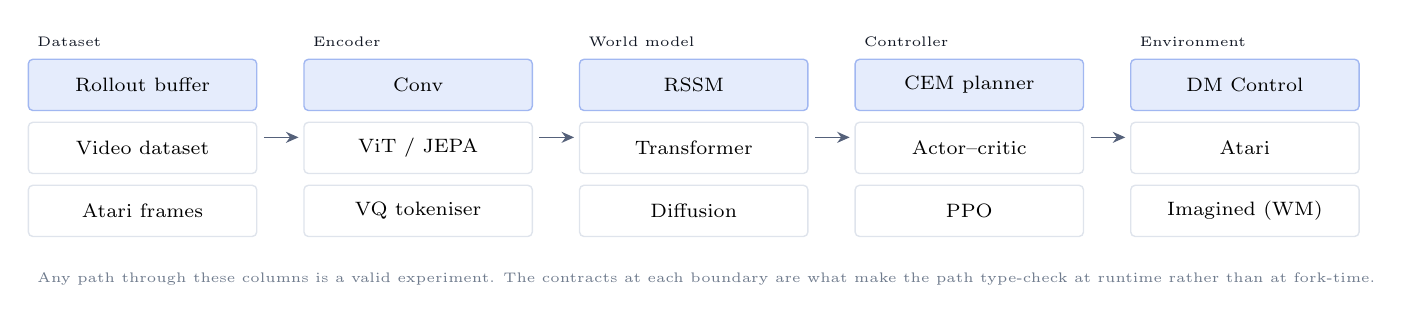
\begin{tikzpicture}[x=1mm,y=1mm,font=\tiny]
  \foreach \i/\slot/\a/\b/\c in {
     0/{Dataset}/{Rollout buffer}/{Video dataset}/{Atari frames},
     1/{Encoder}/{Conv}/{ViT / JEPA}/{VQ tokeniser},
     2/{World model}/{RSSM}/{Transformer}/{Diffusion},
     3/{Controller}/{CEM planner}/{Actor–critic}/{PPO},
     4/{Environment}/{DM Control}/{Atari}/{Imagined (WM)}}{
    \node[anchor=north west,font=\tiny\displayfont,color=ink] at (\i*35,3) {\slot};
    \node[abox,minimum width=29mm,minimum height=6.5mm,anchor=north west] at (\i*35,-1) {\a};
    \node[lbox,minimum width=29mm,minimum height=6.5mm,anchor=north west] at (\i*35,-9) {\b};
    \node[lbox,minimum width=29mm,minimum height=6.5mm,anchor=north west] at (\i*35,-17) {\c};
    \ifnum\i<4 \draw[arr] (\i*35+30,-11) -- (\i*35+34.4,-11); \fi
  }
  \node[anchor=north west,font=\tiny,color=muted] at (0,-27)
    {Any path through these columns is a valid experiment. The contracts at each boundary are what make the path type-check at runtime rather than at fork-time.};
\end{tikzpicture}
\end{center}

\vspace{2mm}
\begin{multicols}{2}
{\footnotesize
\subhead{What this buys a researcher}
\begin{itemize}
  \item \textbf{Swap world models} without rewriting the data pipeline or the environment stack.
  \item \textbf{Change environments}, from pixels to state or simulator to imagined rollout, behind one selector.
  \item \textbf{Benchmark fairly}, because seeds, episode counts, and aggregation come from shared code rather than each paper's script.
  \item \textbf{Reproduce} from a serialisable config plus a registry name.
  \item \textbf{Implement something new} by satisfying one contract, then inherit training, logging, checkpointing, export, and evaluation.
  \item \textbf{Publish it} through the plugin registry, so a third-party model is a first-class citizen of \texttt{create\_model()}.
\end{itemize}}
\end{multicols}

\newpage
% =========================================================== PAGE 5 =========
\pagetitle{Progress}{What exists, what does not}

{\footnotesize
The repository has been under continuous development since November 2025: 593 commits, roughly
37{,}700 lines of library code across 158 modules, and 819 tests in \texttt{tests/} plus a separate
benchmark test suite. Seven releases have been published to PyPI (latest 0.4.2; version 0.5.0 sits
in the repository unreleased). The work is overwhelmingly by a single maintainer.}

\vspace{4mm}

\begin{minipage}[t]{0.325\textwidth}
\begin{tcolorbox}[enhanced,colback=greensoft!45,colframe=green!35,boxrule=0.6pt,arc=2pt,
  left=3mm,right=3mm,top=2.5mm,bottom=2.5mm,height=97mm]
{\displayfont\color{green}\footnotesize IMPLEMENTED}\par\vspace{2mm}
{\scriptsize
\begin{itemize}[label=\textcolor{green}{\scriptsize$\bullet$},leftmargin=3.2mm]
  \item Unified factory API: \texttt{create\_config} / \texttt{create\_model} / \texttt{make\_env}, with 13 registered model families
  \item Dreamer v1/v2/v3, PlaNet, IRIS, JEPA, DIAMOND, DiT, Genie (3 sizes), ModularRSSM
  \item 11 environment backends (Gym, ALE, DMC, MuJoCo, Robotics, Procgen, DMLab, Brax, bsuite, Unity, world-model)
  \item Normalised \texttt{step()} \texttt{info} contract with cross-backend contract tests
  \item \texttt{WorldModelEnv}: trained dynamics model exposed as a \texttt{gym.Env}
  \item Encoders/decoders, VQ layer, video tokeniser, RSSM, MDN-RNN, ViT, DDPM/DiT backbones
  \item Replay/memory modules, dataclass configs with YAML experiment files, serialisation
  \item Benchmark harness: adapters, multi-seed runner, IQM + bootstrap CI, JSON/CSV/Markdown reports; FID, FVD, LPIPS, PSNR
  \item Export to ONNX, TorchScript, TensorRT; plugin registry for third-party models and backends
  \item CLI (\texttt{train\,/\,eval\,/\,benchmark\,/\,play}), Docker image, 52 documentation pages
  \item CI: tests, mypy, lint, CodeQL, docs, PyPI publish; PEP 561 typing stubs
\end{itemize}}
\end{tcolorbox}
\end{minipage}\hfill
\begin{minipage}[t]{0.325\textwidth}
\begin{tcolorbox}[enhanced,colback=ambersoft!55,colframe=amber!35,boxrule=0.6pt,arc=2pt,
  left=3mm,right=3mm,top=2.5mm,bottom=2.5mm,height=97mm]
{\displayfont\color{amber}\footnotesize IN PROGRESS}\par\vspace{2mm}
{\scriptsize
\begin{itemize}[label=\textcolor{amber}{\scriptsize$\bullet$},leftmargin=3.2mm]
  \item \textbf{Uniform training entry point.} Construction is unified across all 13 model families, but a shared step-budget \texttt{train()} currently covers the Dreamer family and a subset of others. Each remaining family still has its own trainer module.
  \item \textbf{Uniform evaluation entry point.} \texttt{evaluate()} exists on some agents; the benchmark adapters paper over the rest.
  \item \textbf{Paper-alignment verification.} Test suites pinning implementations to their papers' appendices exist for IRIS, DiT, and Genie; other families are not yet covered.
  \item \textbf{Dataset abstraction.} Rollout, sequence, and video datasets exist, but there is no single dataset contract every trainer consumes.
  \item \textbf{Multimodal observations} beyond pixels + proprioceptive vectors.
  \item \textbf{Minecraft / open-world environment} adapter.
  \item \textbf{Reference results.} The benchmark harness runs; no reproduced published numbers have been produced or validated yet.
\end{itemize}}
\end{tcolorbox}
\end{minipage}\hfill
\begin{minipage}[t]{0.325\textwidth}
\begin{tcolorbox}[enhanced,colback=slatesoft!60,colframe=slate!25,boxrule=0.6pt,arc=2pt,
  left=3mm,right=3mm,top=2.5mm,bottom=2.5mm,height=97mm]
{\displayfont\color{slate}\footnotesize PLANNED}\par\vspace{2mm}
{\scriptsize
\begin{itemize}[label=\textcolor{slate}{\scriptsize$\bullet$},leftmargin=3.2mm]
  \item Single \texttt{Trainer} / \texttt{evaluate} surface spanning every registered family (the proposed API on page 4)
  \item Published, seed-controlled reference results with confidence intervals for each implemented family
  \item Standard dataset contract plus conversion tools for common trajectory formats
  \item Cross-model, cross-environment leaderboard generated by the benchmark harness
  \item Distributed and multi-GPU training paths
  \item Documented model/dataset hub so third-party components are installable and discoverable
  \item Robotics-oriented environments and sim-to-real evaluation protocol
  \item Community contribution process for models, adapters, and benchmark tasks
\end{itemize}}
\end{tcolorbox}
\end{minipage}

\vspace{5mm}
\sectionhead{Early researcher validation}

\begin{callout}
{\footnotesize
The problem framing and architecture described in this report have been discussed directly with
researchers and engineers working on world models and embodied AI at organisations including
\textbf{Google DeepMind}, \textbf{Odyssey}, \textbf{General Intuition}, and \textbf{Kog AI}. The
reactions to the project were encouraging, and the conversations supported the premise that
infrastructure fragmentation and duplicated engineering are real, felt costs in this area of
research.
\vspace{2mm}

\textbf{What these conversations were, precisely:} informal technical discussions with individual
researchers. They are reported here as \emph{feedback and problem validation only}. They are not
partnerships, endorsements, sponsorships, customer relationships, or any form of official
organisational support. None of the organisations named has reviewed, approved, or endorsed
TorchWM, and no individual is quoted in this document.
\vspace{2mm}

\textbf{How the feedback shaped the project:} it reinforced three decisions that are visible in the
architecture: (i) treating the environment interface as a hard contract with normalised
termination and discount semantics, because wrapper divergence is a recurring source of
irreproducibility; (ii) making the trained world model usable as an ordinary environment, so that
model learning and policy learning stay decoupled; and (iii) prioritising a benchmark harness with
proper aggregate statistics (IQM, bootstrap confidence intervals) over headline single-seed
numbers.}
\end{callout}

\vspace{3mm}
\begin{warncallout}
{\footnotesize\textbf{Stated plainly:} TorchWM has no measured adoption, no published benchmark
results, no external funding, and one primary maintainer. The case for it rests on the problem
being real and the design being sound, not on traction that does not yet exist.}
\end{warncallout}

\newpage
% =========================================================== PAGE 6 =========
\pagetitle{Roadmap}{From library to infrastructure}

{\footnotesize
The phases below are sequenced by dependency, not by date. Each one is only worth starting when the
previous one is solid enough to build on; publishing benchmark numbers before the training paths are
uniform, for example, would produce exactly the incomparable results the project exists to fix.}

\vspace{5mm}

\begin{center}
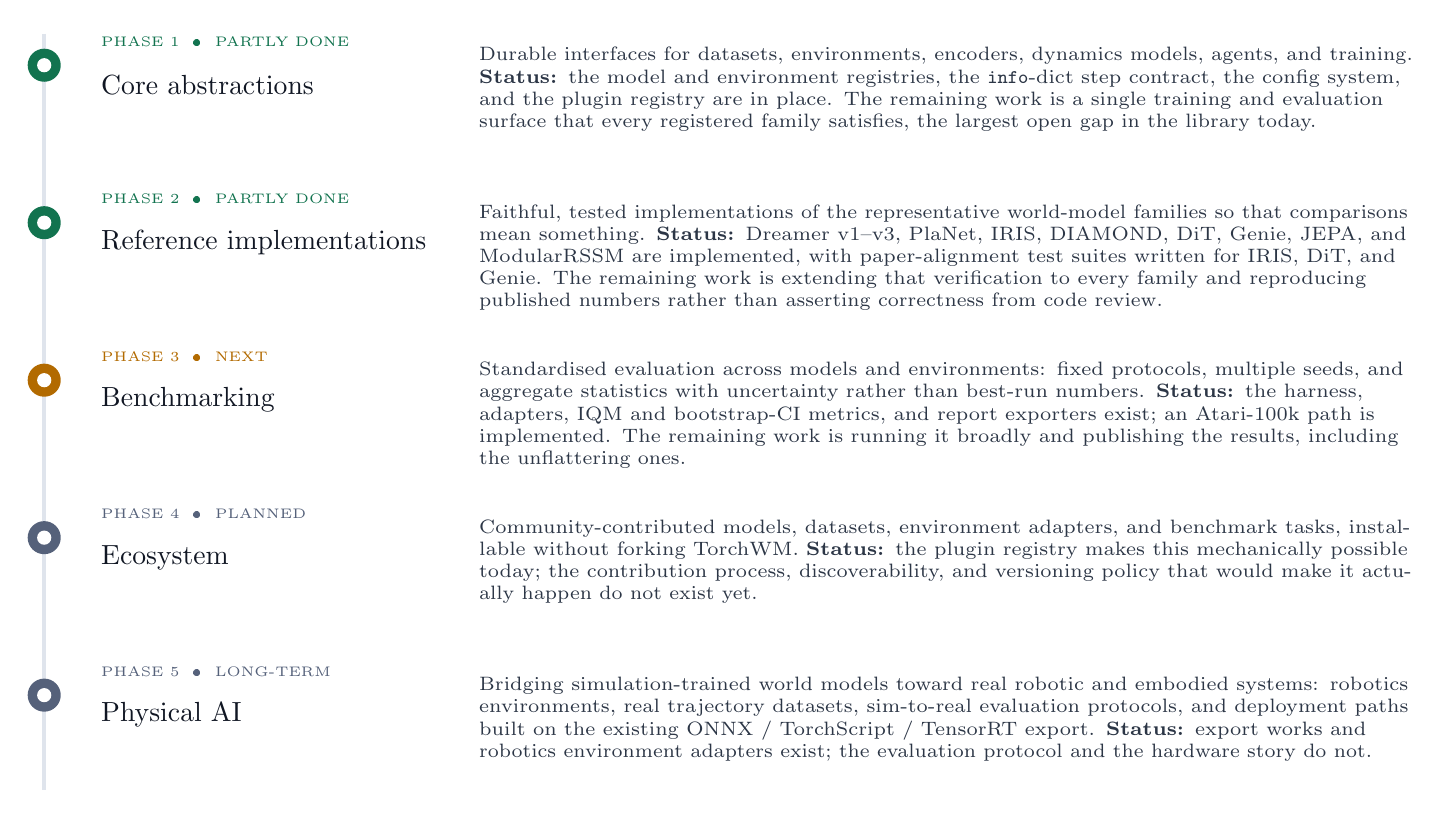
\begin{tikzpicture}[x=1mm,y=1mm,font=\scriptsize]
  \draw[rule,line width=1.4pt] (4,0) -- (4,-96);

  \foreach \i/\ph/\title/\stat/\col in {
    0/{Phase 1}/{Core abstractions}/{partly done}/{green},
    1/{Phase 2}/{Reference implementations}/{partly done}/{green},
    2/{Phase 3}/{Benchmarking}/{next}/{amber},
    3/{Phase 4}/{Ecosystem}/{planned}/{slate},
    4/{Phase 5}/{Physical AI}/{long-term}/{slate}}{
    \fill[\col] (4,-\i*20-4) circle (2.1mm);
    \fill[white] (4,-\i*20-4) circle (0.9mm);
    \node[anchor=west,font=\tiny\displayfont,color=\col] at (10,-\i*20-1) {\MakeUppercase{\ph} \ \textbullet\ \ \MakeUppercase{\stat}};
    \node[anchor=west,font=\normalsize\displayfont,color=ink] at (10,-\i*20-6.5) {\title};
  }

  % descriptions
  \node[anchor=north west,text width=118mm,font=\scriptsize,color=body] at (58,-0.5)
    {Durable interfaces for datasets, environments, encoders, dynamics models, agents, and training.
     \textbf{Status:} the model and environment registries, the \texttt{info}-dict step contract, the
     config system, and the plugin registry are in place. The remaining work is a single training and
     evaluation surface that every registered family satisfies, the largest open gap in the library today.};

  \node[anchor=north west,text width=118mm,font=\scriptsize,color=body] at (58,-20.5)
    {Faithful, tested implementations of the representative world-model families so that comparisons
     mean something. \textbf{Status:} Dreamer v1--v3, PlaNet, IRIS, DIAMOND, DiT, Genie, JEPA, and
     ModularRSSM are implemented, with paper-alignment test suites written for IRIS, DiT, and Genie.
     The remaining work is extending that verification to every family and reproducing published
     numbers rather than asserting correctness from code review.};

  \node[anchor=north west,text width=118mm,font=\scriptsize,color=body] at (58,-40.5)
    {Standardised evaluation across models and environments: fixed protocols, multiple seeds, and
     aggregate statistics with uncertainty rather than best-run numbers. \textbf{Status:} the harness,
     adapters, IQM and bootstrap-CI metrics, and report exporters exist; an Atari-100k path is
     implemented. The remaining work is running it broadly and publishing the results, including the
     unflattering ones.};

  \node[anchor=north west,text width=118mm,font=\scriptsize,color=body] at (58,-60.5)
    {Community-contributed models, datasets, environment adapters, and benchmark tasks, installable
     without forking TorchWM. \textbf{Status:} the plugin registry makes this mechanically possible
     today; the contribution process, discoverability, and versioning policy that would make it
     actually happen do not exist yet.};

  \node[anchor=north west,text width=118mm,font=\scriptsize,color=body] at (58,-80.5)
    {Bridging simulation-trained world models toward real robotic and embodied systems: robotics
     environments, real trajectory datasets, sim-to-real evaluation protocols, and deployment paths
     built on the existing ONNX / TorchScript / TensorRT export. \textbf{Status:} export works and
     robotics environment adapters exist; the evaluation protocol and the hardware story do not.};
\end{tikzpicture}
\end{center}

\vspace{4mm}

\begin{accentcallout}
{\subhead{The larger vision}
\footnotesize
World models sit at the intersection of four communities that currently share very little code:
representation learning, model-based reinforcement learning, simulation, and robotics. Each has its
own conventions for what an observation is, what an action is, what a rollout is, and what counts as
a result. A world model needs all four at once, which is why it is the natural place for a shared
infrastructure layer to form.
\vspace{2mm}

TorchWM's long-term goal is to be that layer: a common substrate where a dynamics model trained on
video can be evaluated as a simulator, used as an environment for policy learning, benchmarked
against alternatives under a fixed protocol, and exported toward a physical system, without any of
those steps requiring a rewrite. \bvis}
\end{accentcallout}

\vspace{4mm}
\sectionhead{Open questions the design still has to answer}

\begin{center}
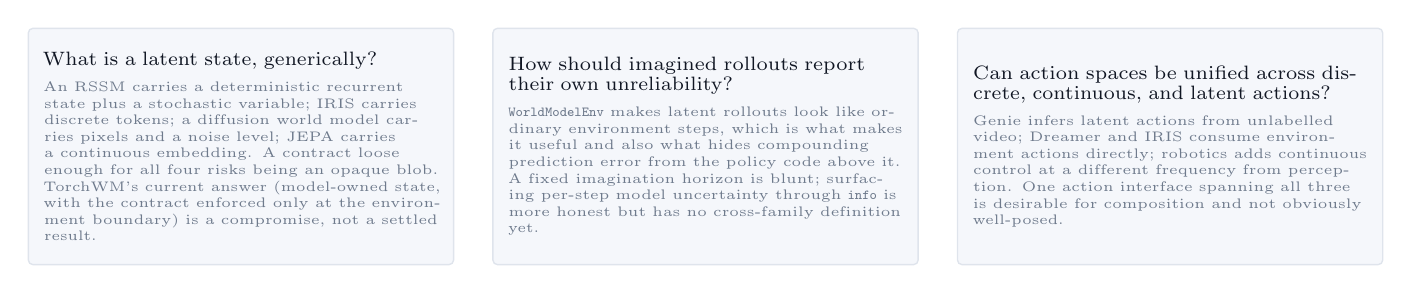
\begin{tikzpicture}[x=1mm,y=1mm,font=\scriptsize]
  \foreach \i/\q/\d in {
    0/{What is a latent state, generically?}/{An RSSM carries a deterministic recurrent state plus a stochastic variable; IRIS carries discrete tokens; a diffusion world model carries pixels and a noise level; JEPA carries a continuous embedding. A contract loose enough for all four risks being an opaque blob. TorchWM's current answer (model-owned state, with the contract enforced only at the environment boundary) is a compromise, not a settled result.},
    1/{How should imagined rollouts report their own unreliability?}/{\texttt{WorldModelEnv} makes latent rollouts look like ordinary environment steps, which is what makes it useful and also what hides compounding prediction error from the policy code above it. A fixed imagination horizon is blunt; surfacing per-step model uncertainty through \texttt{info} is more honest but has no cross-family definition yet.},
    2/{Can action spaces be unified across discrete, continuous, and latent actions?}/{Genie infers latent actions from unlabelled video; Dreamer and IRIS consume environment actions directly; robotics adds continuous control at a different frequency from perception. One action interface spanning all three is desirable for composition and not obviously well-posed.}}{
    \node[lbox,fill=panel,draw=rule,minimum width=54mm,minimum height=30mm,anchor=north west,text width=50mm,align=left,font=\tiny]
      at (\i*59,0) {{\scriptsize\displayfont\color{ink}\q}\\[1.2mm]{\color{muted}\d}};
  }
\end{tikzpicture}
\end{center}

\newpage
% =========================================================== PAGE 7 =========
\pagetitle{Positioning}{Where TorchWM fits, and where it does not}

{\footnotesize
Adjacent efforts exist and are worth taking seriously. TorchWM's case does not rest on being alone
in the space; it rests on covering a combination the existing tools do not.}

\vspace{3mm}

{\footnotesize
\begin{tabular}{@{}p{0.20\textwidth}p{0.40\textwidth}p{0.36\textwidth}@{}}
\toprule
\textbf{Effort} & \textbf{Focus} & \textbf{Relationship to TorchWM}\\
\midrule
Gymnasium [1] & Standard environment interface for RL. & A dependency and a model. TorchWM adopts its step semantics and extends them with a normalised \texttt{info} contract across nine backends.\\[1.4mm]
MBRL-Lib [2] & Modular model-based RL toolbox: dynamics models, planners, MBRL algorithms. & Closest in spirit for the control half. TorchWM spans a wider model space: token-based, diffusion, and video world models, not only proprioceptive MBRL.\\[1.4mm]
TorchRL [3] & General PyTorch RL library with tensor-first data structures. & Complementary. TorchWM's \texttt{WorldModelEnv} lets an imagined environment be consumed by external RL libraries rather than replacing them.\\[1.4mm]
stable-worldmodel [4] & Reproducible world-modelling platform: Lance data layer, planning solvers, controlled factors of variation. & Nearest neighbour. Strongest on data infrastructure and MPC-style planning evaluation; TorchWM is broader on model families and the agent/policy side, and PyTorch-native throughout.\\[1.4mm]
OpenWorldLib [5] & Unified codebase and definition spanning generative, reasoning, and interactive world models. & Broader in the generative/multimodal direction; less focused on the reinforcement-learning and control loop that TorchWM centres.\\[1.4mm]
WorldArena [8] and related benchmarks & Evaluation suites for embodied world models. & Evaluation targets rather than infrastructure. TorchWM's harness is meant to run against suites like these, not compete with them.\\
\bottomrule
\end{tabular}}

\vspace{4mm}
\begin{callout}
{\footnotesize
\subhead{Where TorchWM could differentiate}
\begin{itemize}
  \item \textbf{Breadth of model families under one registry.} Recurrent state-space, transformer/token, diffusion, and joint-embedding predictive models are reachable through the same factory, a span most alternatives do not attempt.
  \item \textbf{The world model as an environment.} Making imagination a \texttt{gym.Env} keeps model learning and policy learning independently replaceable, and lets external RL code operate on learned dynamics unmodified.
  \item \textbf{PyTorch-native and deployment-aware.} One framework end to end, with ONNX / TorchScript / TensorRT export already in place, an unusual concern for a research library, and the prerequisite for the Physical AI phase.
  \item \textbf{Contracts over conventions.} Termination, truncation, and discount semantics are enforced by tests across every backend rather than documented and hoped for.
\end{itemize}
\vspace{1mm}
None of these is a claim of superiority. They are the axes along which TorchWM is being built, stated so that they can be judged.}
\end{callout}

\vspace{4mm}
\sectionhead{References}

{\scriptsize
\setlength{\columnsep}{7mm}
\begin{multicols}{2}
\begin{enumerate}[leftmargin=5.5mm,itemsep=0.8mm,label={\color{muted}[\arabic*]}]
  \item M. Towers et al. \emph{Gymnasium: A Standard Interface for Reinforcement Learning Environments}. \texttt{arXiv:2407.17032}.
  \item L. Pineda, B. Amos, A. Zhang, N. O. Lambert, R. Calandra. \emph{MBRL-Lib: A Modular Library for Model-Based Reinforcement Learning}. \texttt{arXiv:2104.10159}.
  \item A. Bou et al. \emph{TorchRL: A data-driven decision-making library for PyTorch}. \texttt{arXiv:2306.00577}.
  \item L. Maes, Q. Le Lidec, D. Haramati, N. Massaudi, D. Scieur, Y. LeCun, R. Balestriero. \emph{stable-worldmodel: A Platform for Reproducible World Modeling Research and Evaluation}. \texttt{arXiv:2602.08968} / \texttt{arXiv:2605.21800}.
  \item OpenDCAI. \emph{OpenWorldLib: A Unified Codebase and Definition of Advanced World Models}. \texttt{arXiv:2604.04707}.
  \item \emph{A Comprehensive Survey on World Models for Embodied AI}. \texttt{arXiv:2510.16732}.
  \item \emph{World Models: A Comprehensive Survey of Architectures, Methodologies, Reasoning Paradigms, and Applications}. \texttt{arXiv:2606.00133}.
  \item \emph{WorldArena: A Unified Benchmark for Evaluating Perception and Functional Utility of Embodied World Models}. \texttt{arXiv:2602.08971}.
  \item D. Ha, J. Schmidhuber. \emph{World Models}. NeurIPS 2018. \texttt{arXiv:1803.10122}.
  \item D. Hafner, T. Lillicrap, I. Fischer, R. Villegas, D. Ha, H. Lee, J. Davidson. \emph{Learning Latent Dynamics for Planning from Pixels} (PlaNet). ICML 2019.
  \item D. Hafner, T. Lillicrap, J. Ba, M. Norouzi. \emph{Dream to Control: Learning Behaviors by Latent Imagination} (Dreamer). ICLR 2020.
  \item D. Hafner, J. Pasukonis, J. Ba, T. Lillicrap. \emph{Mastering Diverse Domains through World Models} (DreamerV3). \texttt{arXiv:2301.04104}.
  \item V. Micheli, E. Alonso, F. Fleuret. \emph{Transformers are Sample-Efficient World Models} (IRIS). ICLR 2023.
  \item E. Alonso, A. Jelley, V. Micheli, A. Kanervisto, A. Storkey, T. Pearce, F. Fleuret. \emph{Diffusion for World Modeling: Visual Details Matter in Atari} (DIAMOND). NeurIPS 2024.
  \item J. Bruce et al. \emph{Genie: Generative Interactive Environments}. ICML 2024.
  \item M. Assran et al. \emph{Self-Supervised Learning from Images with a Joint-Embedding Predictive Architecture} (I-JEPA). CVPR 2023.
  \item W. Peebles, S. Xie. \emph{Scalable Diffusion Models with Transformers} (DiT). ICCV 2023.
  \item R. Agarwal, M. Schwarzer, P. S. Castro, A. Courville, M. G. Bellemare. \emph{Deep Reinforcement Learning at the Edge of the Statistical Precipice}. NeurIPS 2021. \emph{(Source of the IQM and bootstrap-CI protocol used in TorchWM's benchmark harness.)}
\end{enumerate}
\end{multicols}}


\end{document}
